\documentclass[10pt]{article}
\usepackage[margin=0.8in]{geometry}
\usepackage{fancyhdr}
\usepackage{hyperref}
\usepackage{graphicx}
\usepackage{lmodern}
\usepackage[T1]{fontenc}
\usepackage[utf8]{inputenc}
\usepackage{dirtree}
\usepackage{float}

\hypersetup{
    colorlinks=true,
    linkcolor=blue,
    urlcolor=blue,
}

\title{\Huge \textbf{Angry Birds} \\ \Large Built with PYGAME}
\author{\textbf{Sparsh Gupta} \\ \textbf{24B1043} \\ \\ CS104 Project Report}
\date{Spring Semester, 2024--2025}

\pagestyle{fancy}
\fancyhf{}
\lhead{Angry Birds - CS104}
\rhead{Sparsh Gupta}
\cfoot{\thepage}

\begin{document}

\maketitle
\vspace{-1em}
\hrule
\vspace{1em}

\begin{abstract}
This report presents the design and development of \textbf{Angry Birds}, a 2D game developed using Python and the PYGAME library. The project is inspired by the classic Angry Birds mechanics and serves as an exploration into basic game physics, collision detection, and gameplay logic. The report discusses the modules used, directory structure, core game features, customizations and challenges faced, with the aim of providing insight into the game's functionality and underlying architecture.
\end{abstract}

\tableofcontents
\newpage

\section{Introduction}
\label{sec:intro}
\textit{Angry Birds} is an interactive 2D game where players launch a bird using a slingshot to destroy their opponent's tower using the minimum possible number of birds. Developed using PYGAME, the game aims to replicate essential elements of physics-driven gameplay such as parabolic motion and impact dynamics.\\
The primary goal of the project was to learn and implement concepts related to object-oriented programming, 2D rendering, input handling, and basic physics. \\ \\
The player can choose between two themes - \textbf{Day Theme} and \textbf{Night Theme}. The theme selection does not alter gameplay mechanics but adds immersion and visual variety.
The game maintains a stable frame rate of 60 FPS (frames per second), ensuring an overall fluid gameplay experience.

\section{Modules Used}
\begin{itemize}
    \item \texttt{pygame-ce} – Core library used for rendering graphics, handling events, audio playback, and game loop management.
    \item \texttt{math} – Provides trigonometric and mathematical functions essential for bird trajectory and slingshot calculations.
    \item \texttt{numpy} – Used for random bird generation.
    \item \texttt{sys} – Handles program exit.
    \item \texttt{time} – Used for time-based interactions, animations and input delay.
\end{itemize}

\section{Project Directory Layout}
The structure of the project is organized for clarity and modularity:
\dirtree{%
    .1 Angry Birds.
    .2 data.
    .3 audio.
    .3 font.
    .3 images.
    .3 leaderboard.txt.
    .3 tower1.txt.
    .3 tower2.txt.
    .2 scripts.
    .3 bird.py.
    .3 block.py.
    .3 tower.py.
    .3 utils.py.
    .2 main.py.
}

\begin{itemize}
    \item \textbf{main.py} – Launches the application, sets up initial game state, controls the game loop, rendering and animations.
    \item \textbf{bird.py} – Contains the Bird class.
    \item \textbf{block.py} – Contains the Block class.
    \item \textbf{tower.py} – Contains the Tower class.
    \item \textbf{utils.py} – Contains utility functions that support core gameplay logic, such as vector and angle calculations, sling action, collision helpers.
\end{itemize}

\section{Running the Game}
\subsection{Requirements}
To run the game, the following setup is required:
\begin{itemize}
    \item Python 3.9 or newer
    \item pygame library
\end{itemize}
Installation can be done via pip:
\begin{verbatim}
pip install pygame
\end{verbatim}

\subsection{Execution}
Navigate to the project directory and run:
\begin{verbatim}
python main.py
\end{verbatim}

\section{Game Navigation and Gameplay}
\subsection{Intro Screen}
The game starts with an intro screen with a loading bar.

\begin{figure}[H]
    \centering
    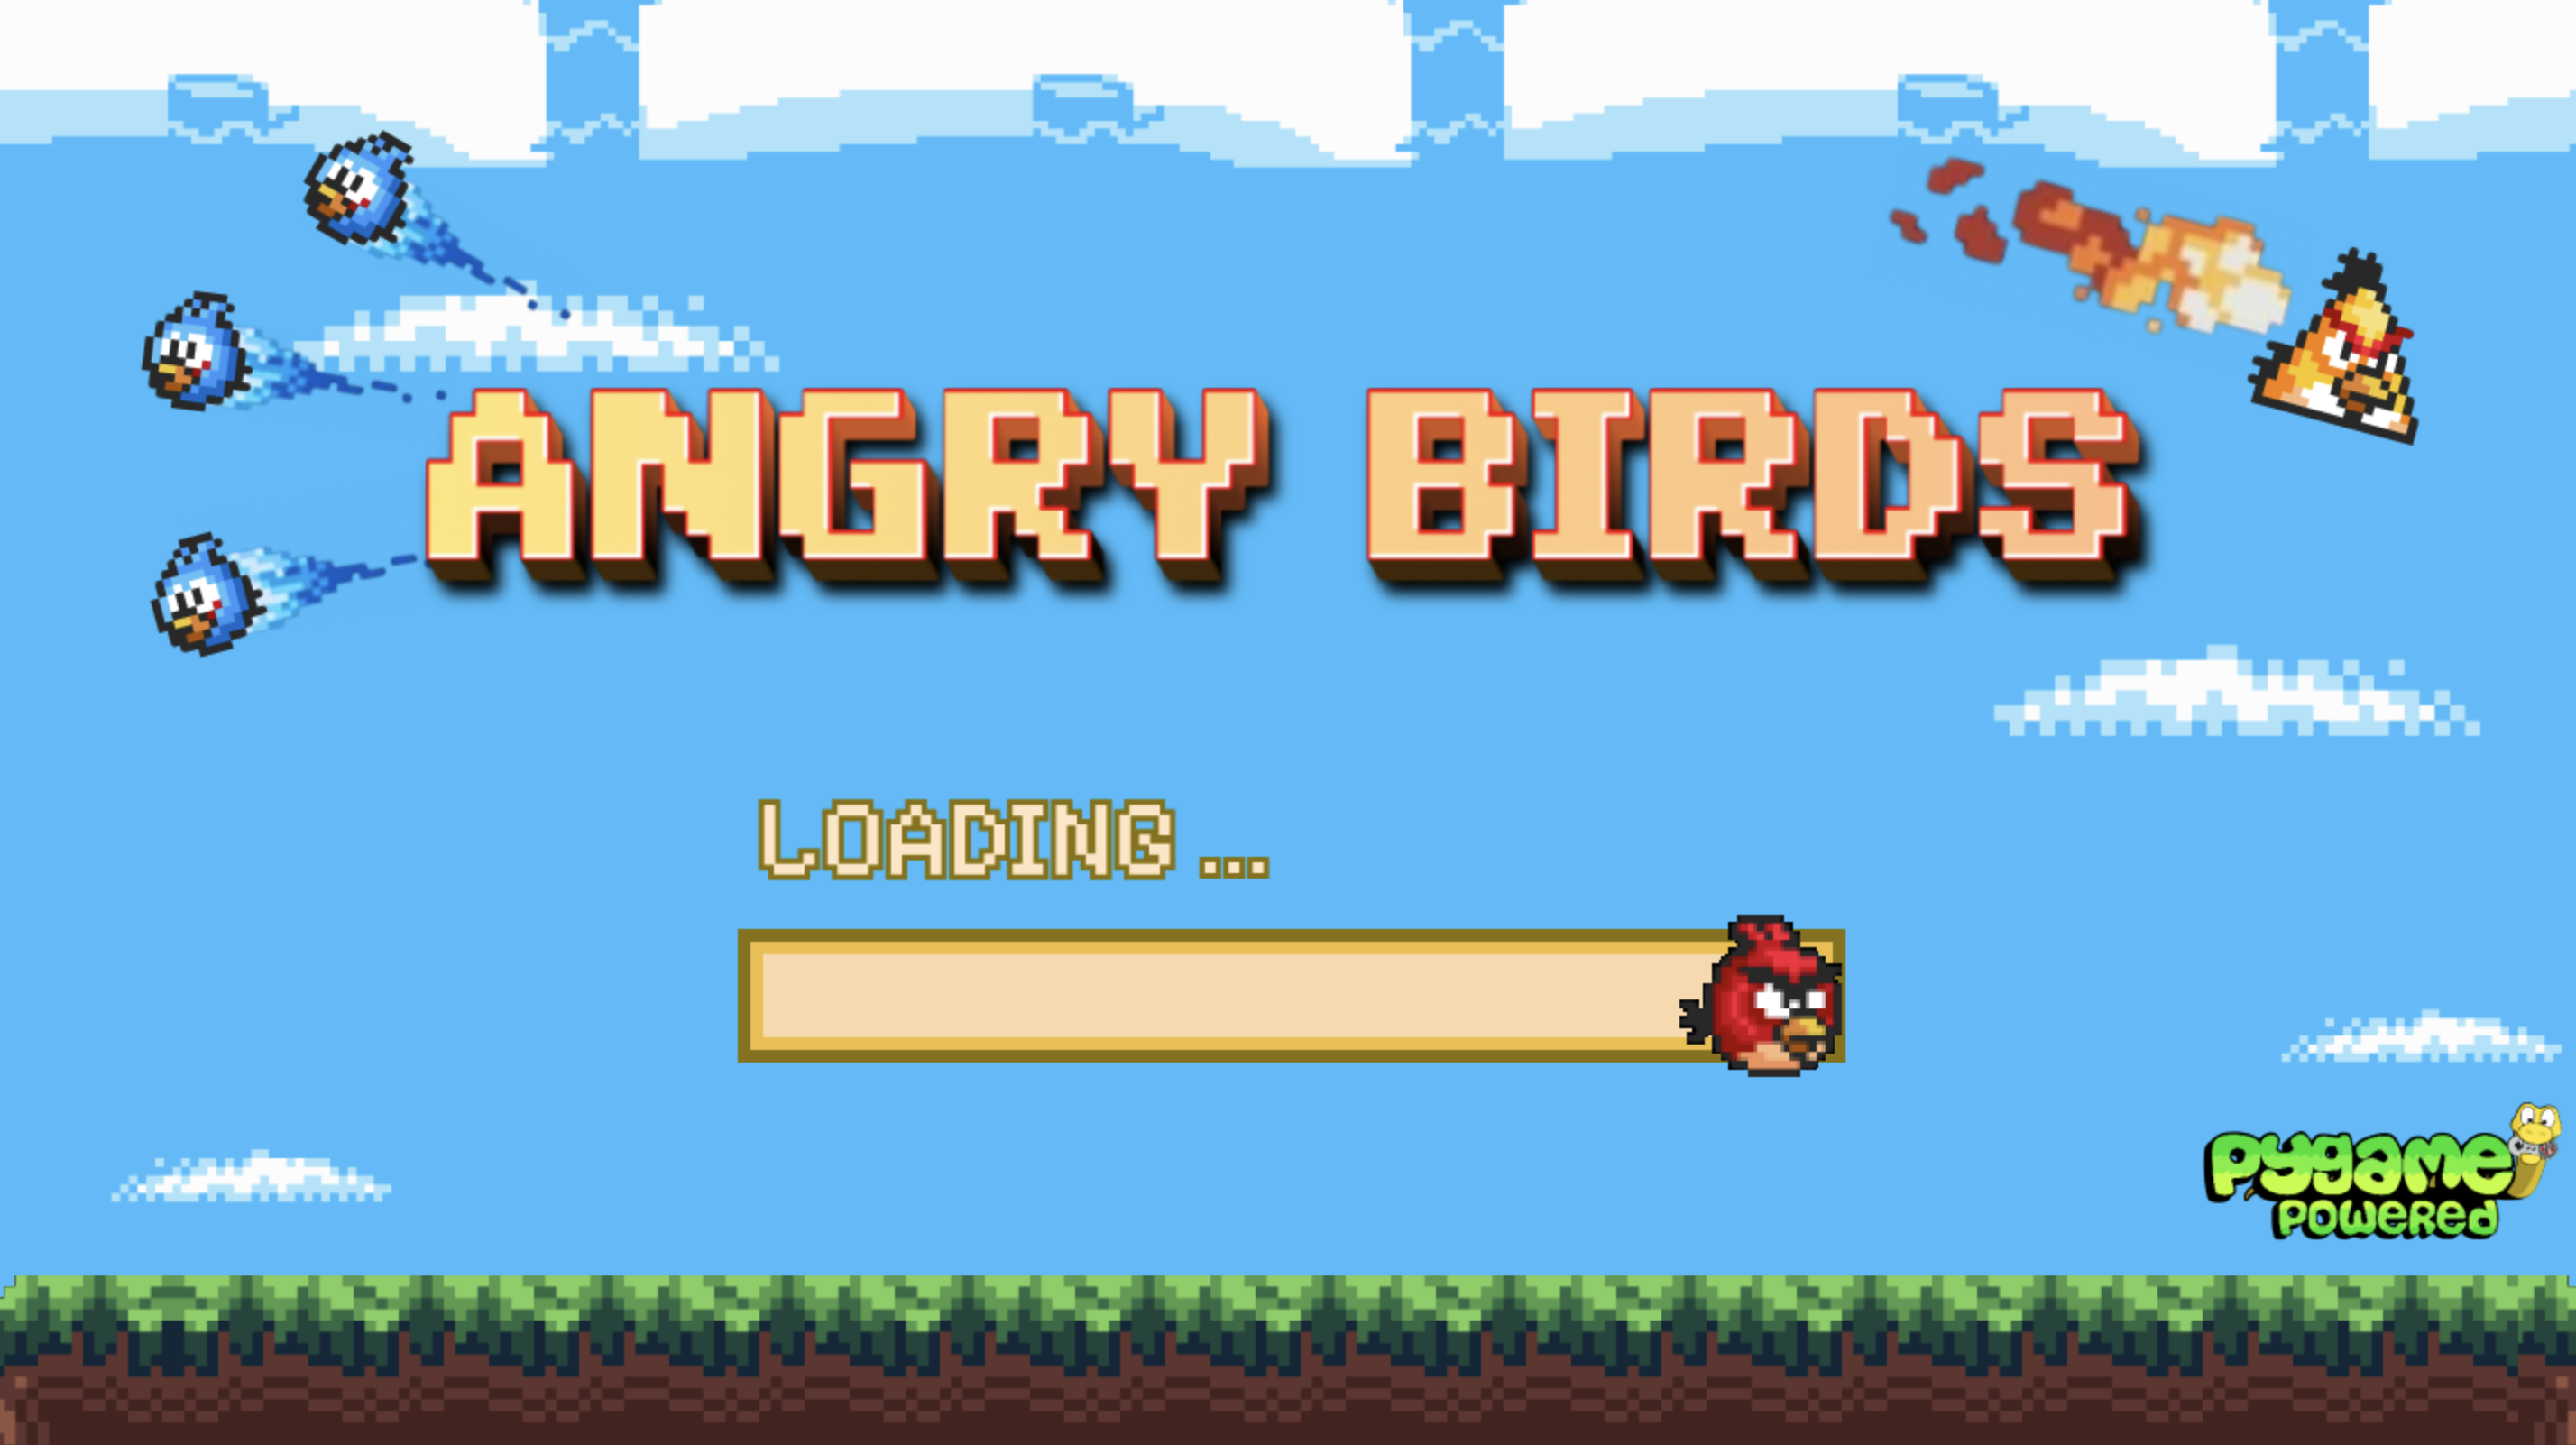
\includegraphics[width=0.5\textwidth]{introscreen.png}
    \caption{Loading Screen}
\end{figure}

\subsection{Main Menu}
Once the loading bar is complete, players are presented with a Main Menu interface offering the following options:

\begin{itemize}
    \item \textbf{Play} – Start the game and proceed to entering player names.
    \item \textbf{leaderboard} – Display names of top 3 players for each mode.
    \item \textbf{Settings} – Toggle sound on/off and Adjust gameplay preferences.
    \item \textbf{Quit} – Quit the game and return to the desktop.
\end{itemize}

These options are accessible using the mouse, and the menu interface is designed to be intuitive and responsive across various screen resolutions.

\begin{figure}[H]
    \centering
    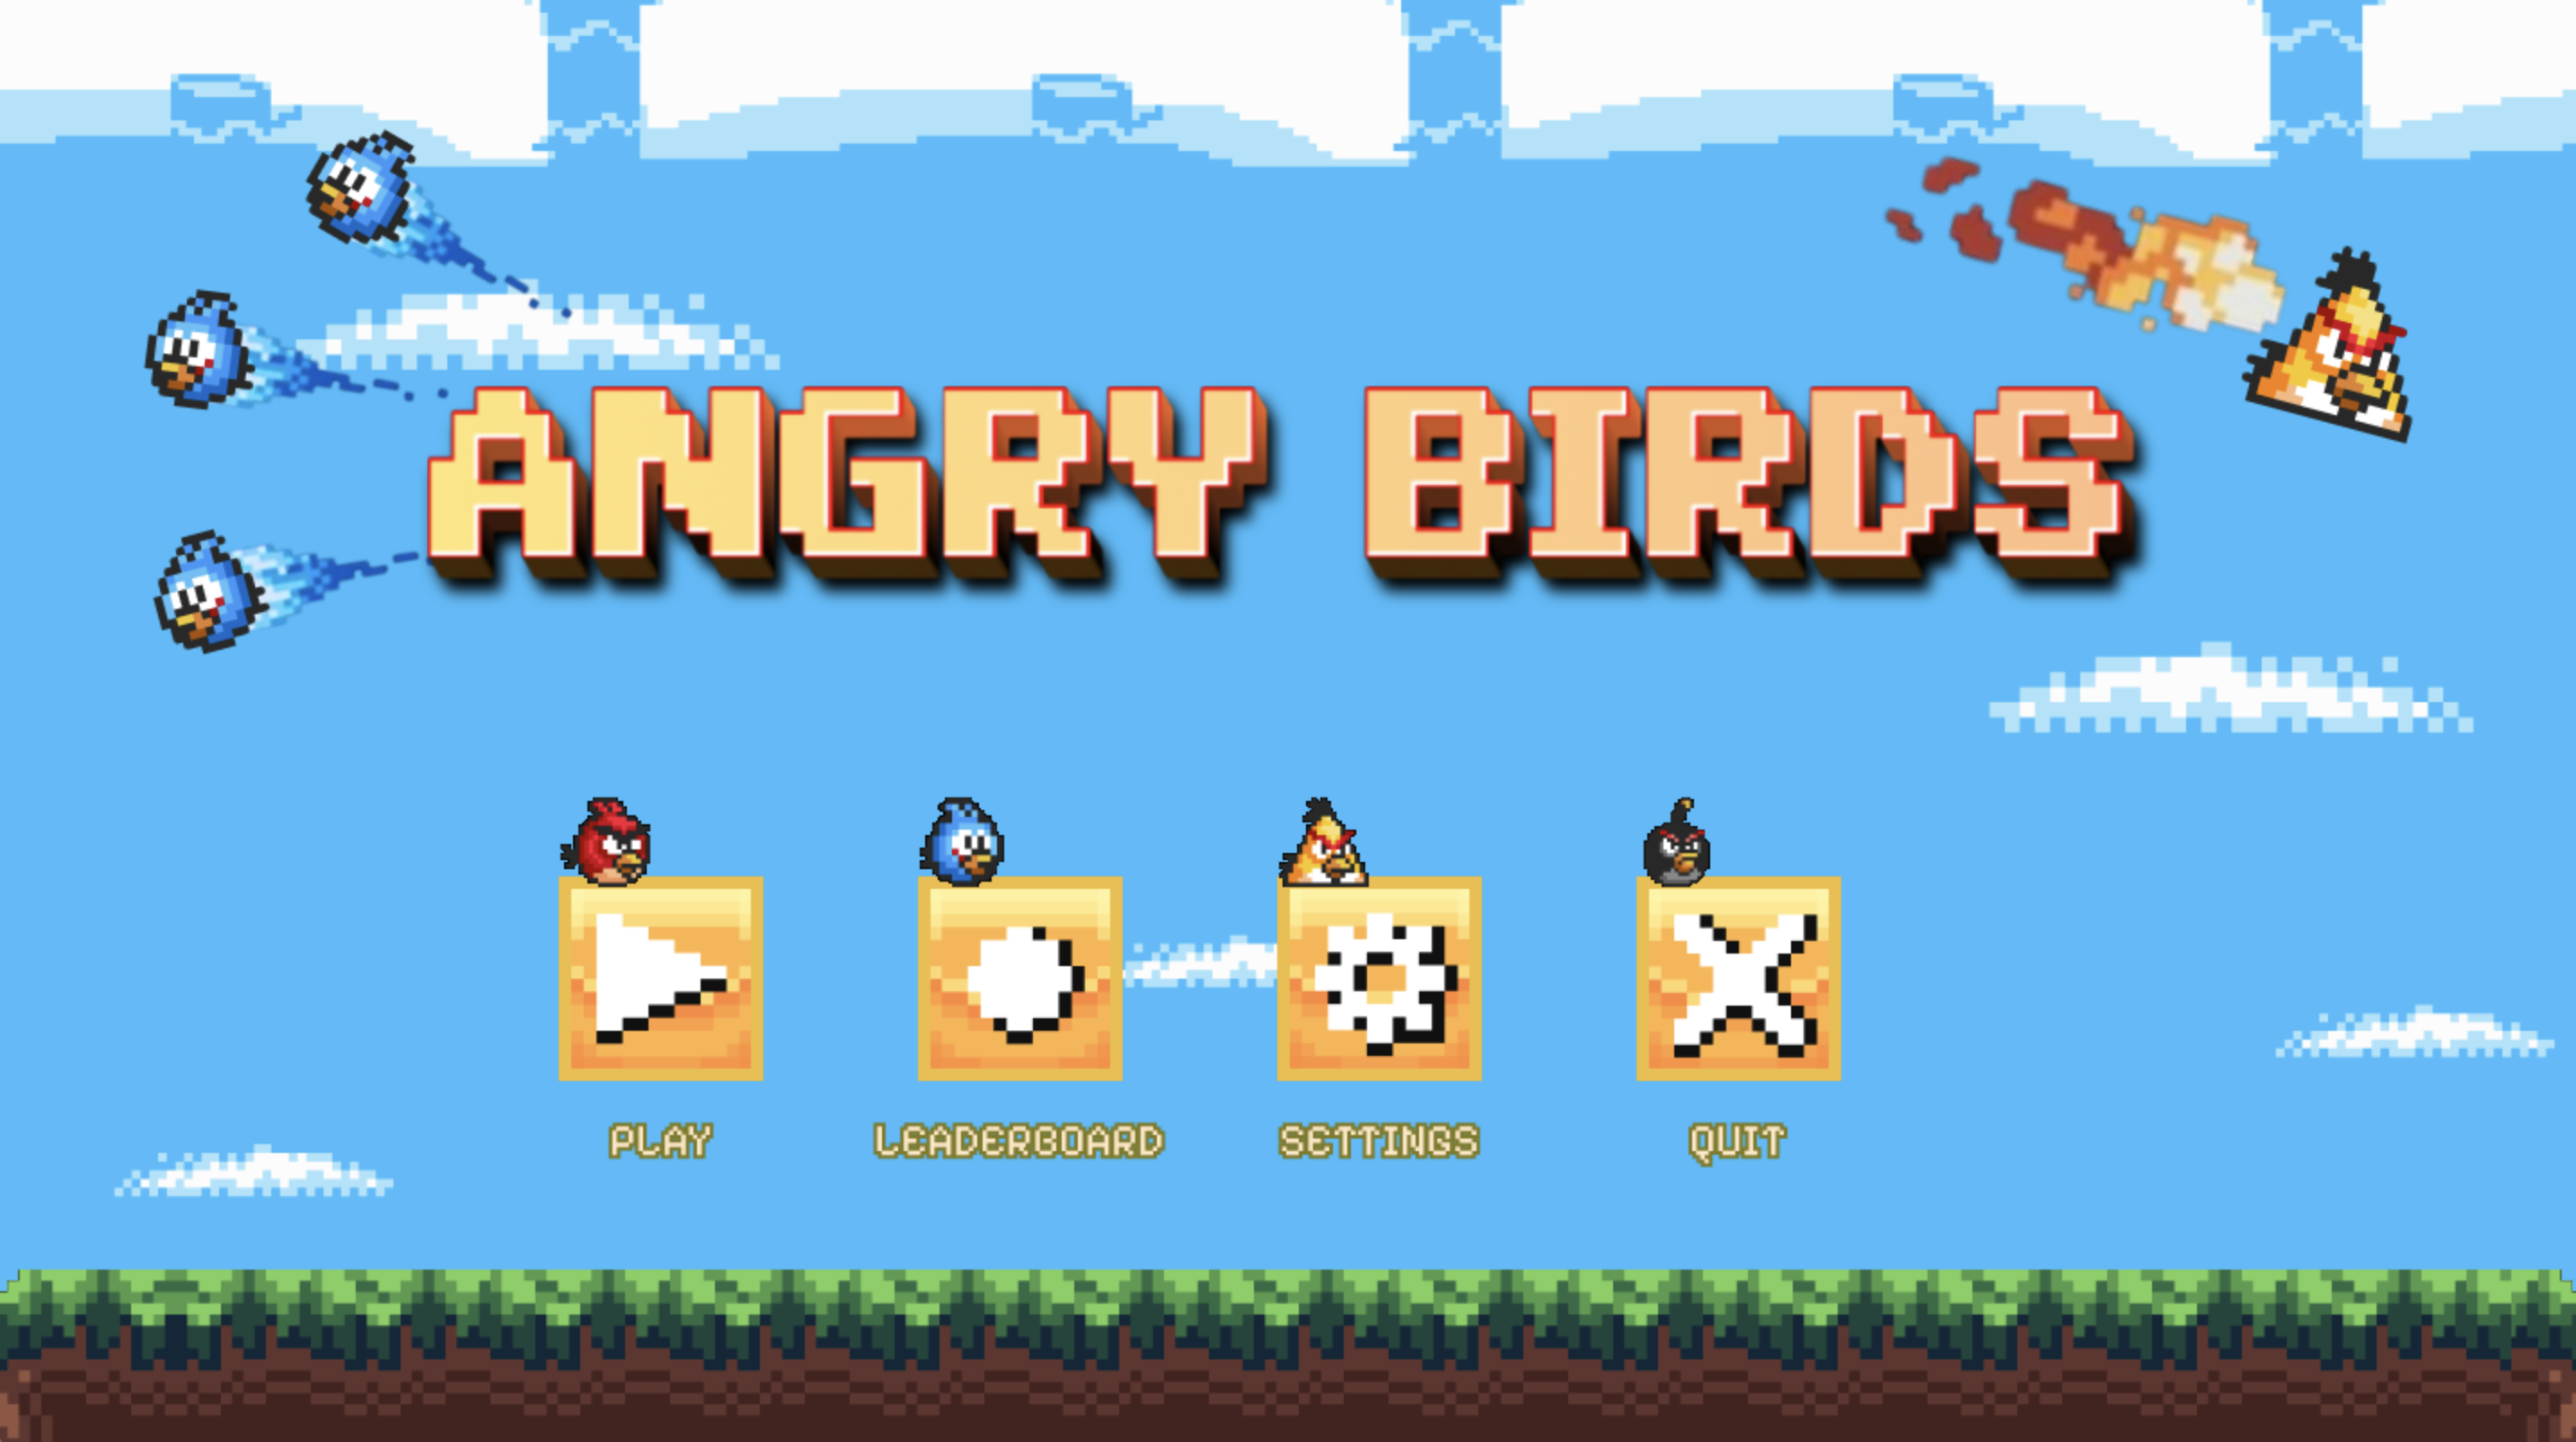
\includegraphics[width=0.5\textwidth]{mainmenu.png}
    \caption{Main Menu}
\end{figure}

\subsection{Enter Player Name}
On clicking the play button, the players are presented with an interface for entering their names.

\begin{figure}[H]
    \centering
    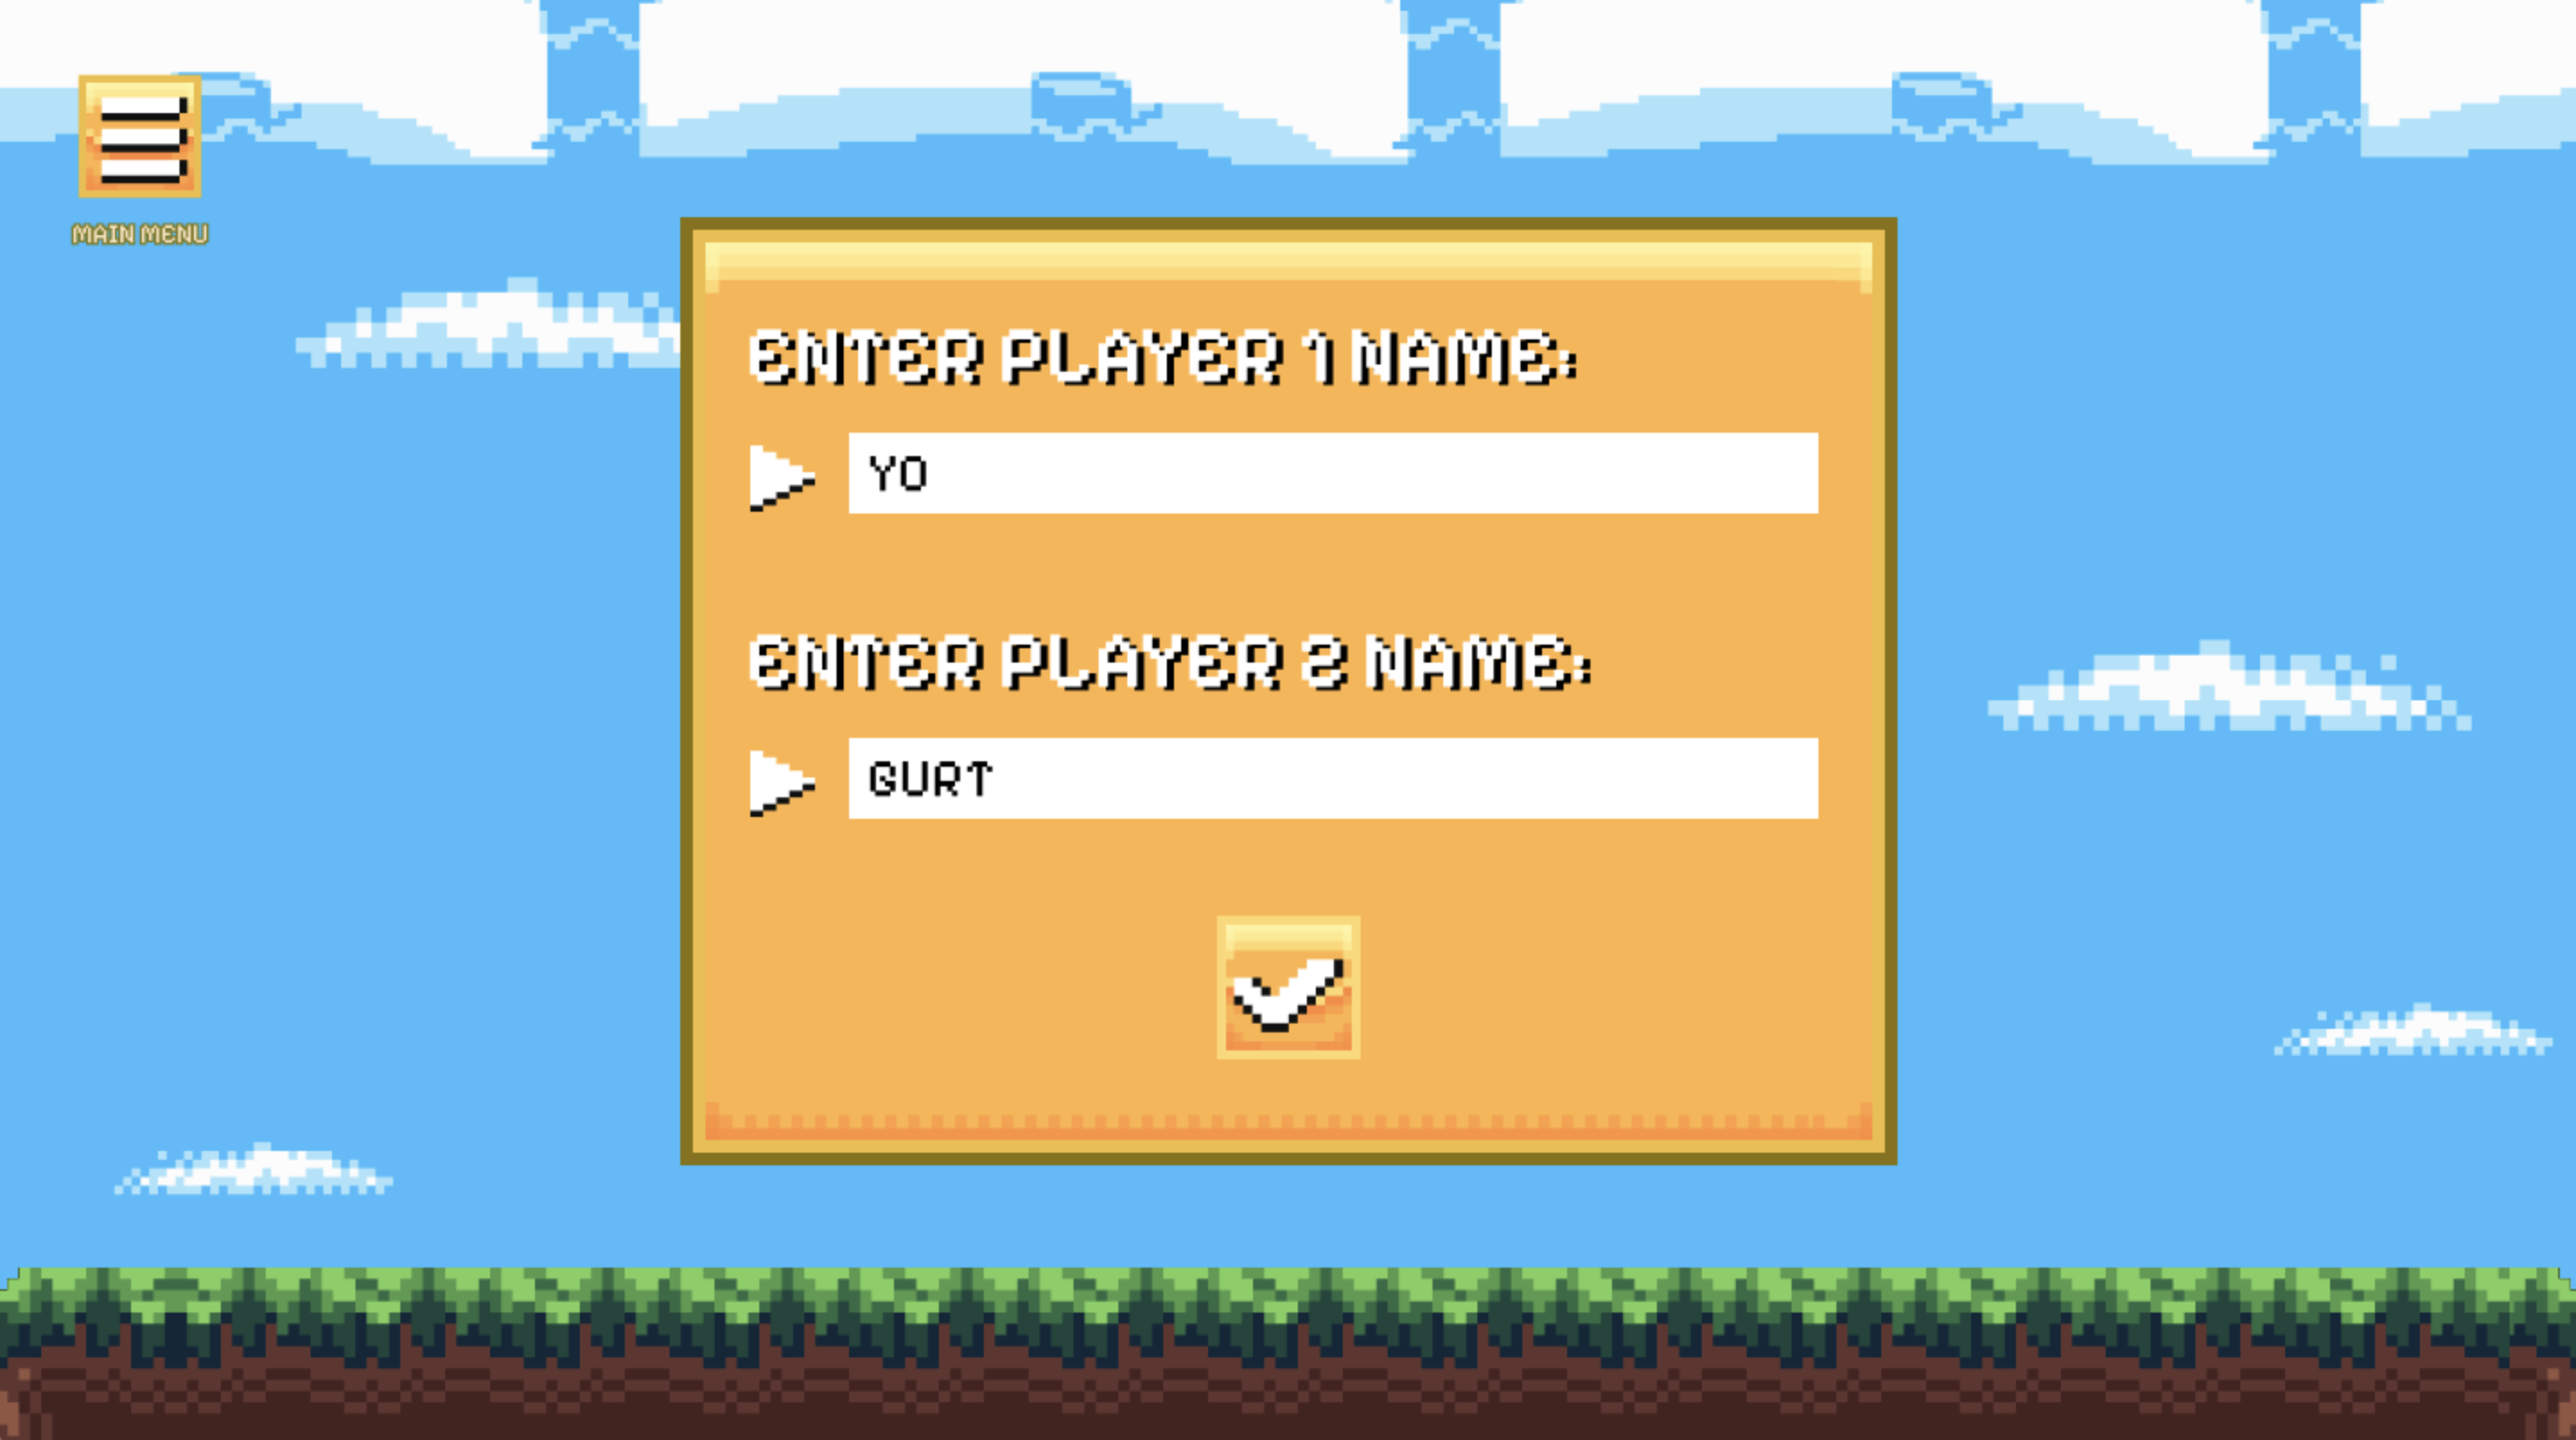
\includegraphics[width=0.5\textwidth]{enterplayername.png}
    \caption{Enter Player Name Screen}
\end{figure}

\subsection{Mode Selection}
After entering player names, the players have to choose among two game modes - One tower mode, Two tower mode.

\subsection{Gameplay}
The player is taken to the selected game mode, where the birds are loaded onto each slingshot. The next bird for each player is generated randomly.
To aim, the player clicks and drags the bird away from the slingshot origin. As the drag vector increases, the stored launch velocity increases proportionally, mimicking a stretched elastic band. Once released, the bird follows a parabolic trajectory.
The player which destoys the other player towers first is declared the winner and his/her leaderboard ranking is calculated using the number of birds used to destroy the tower.
\textit{Trajectory dots} to see the path of the bird before launching and \textit{wind} can be enabled in \textbf{Settings}. \\ \\
Upon impact with a block, the bird's velocity changes according to realistic physics logic. The player which plays first is decided randomly using numpy's random module. A tower consists of one or two columns of blocks with 10 blocks in each column. The health of each block is 100.

\begin{figure}[H]
    \centering
    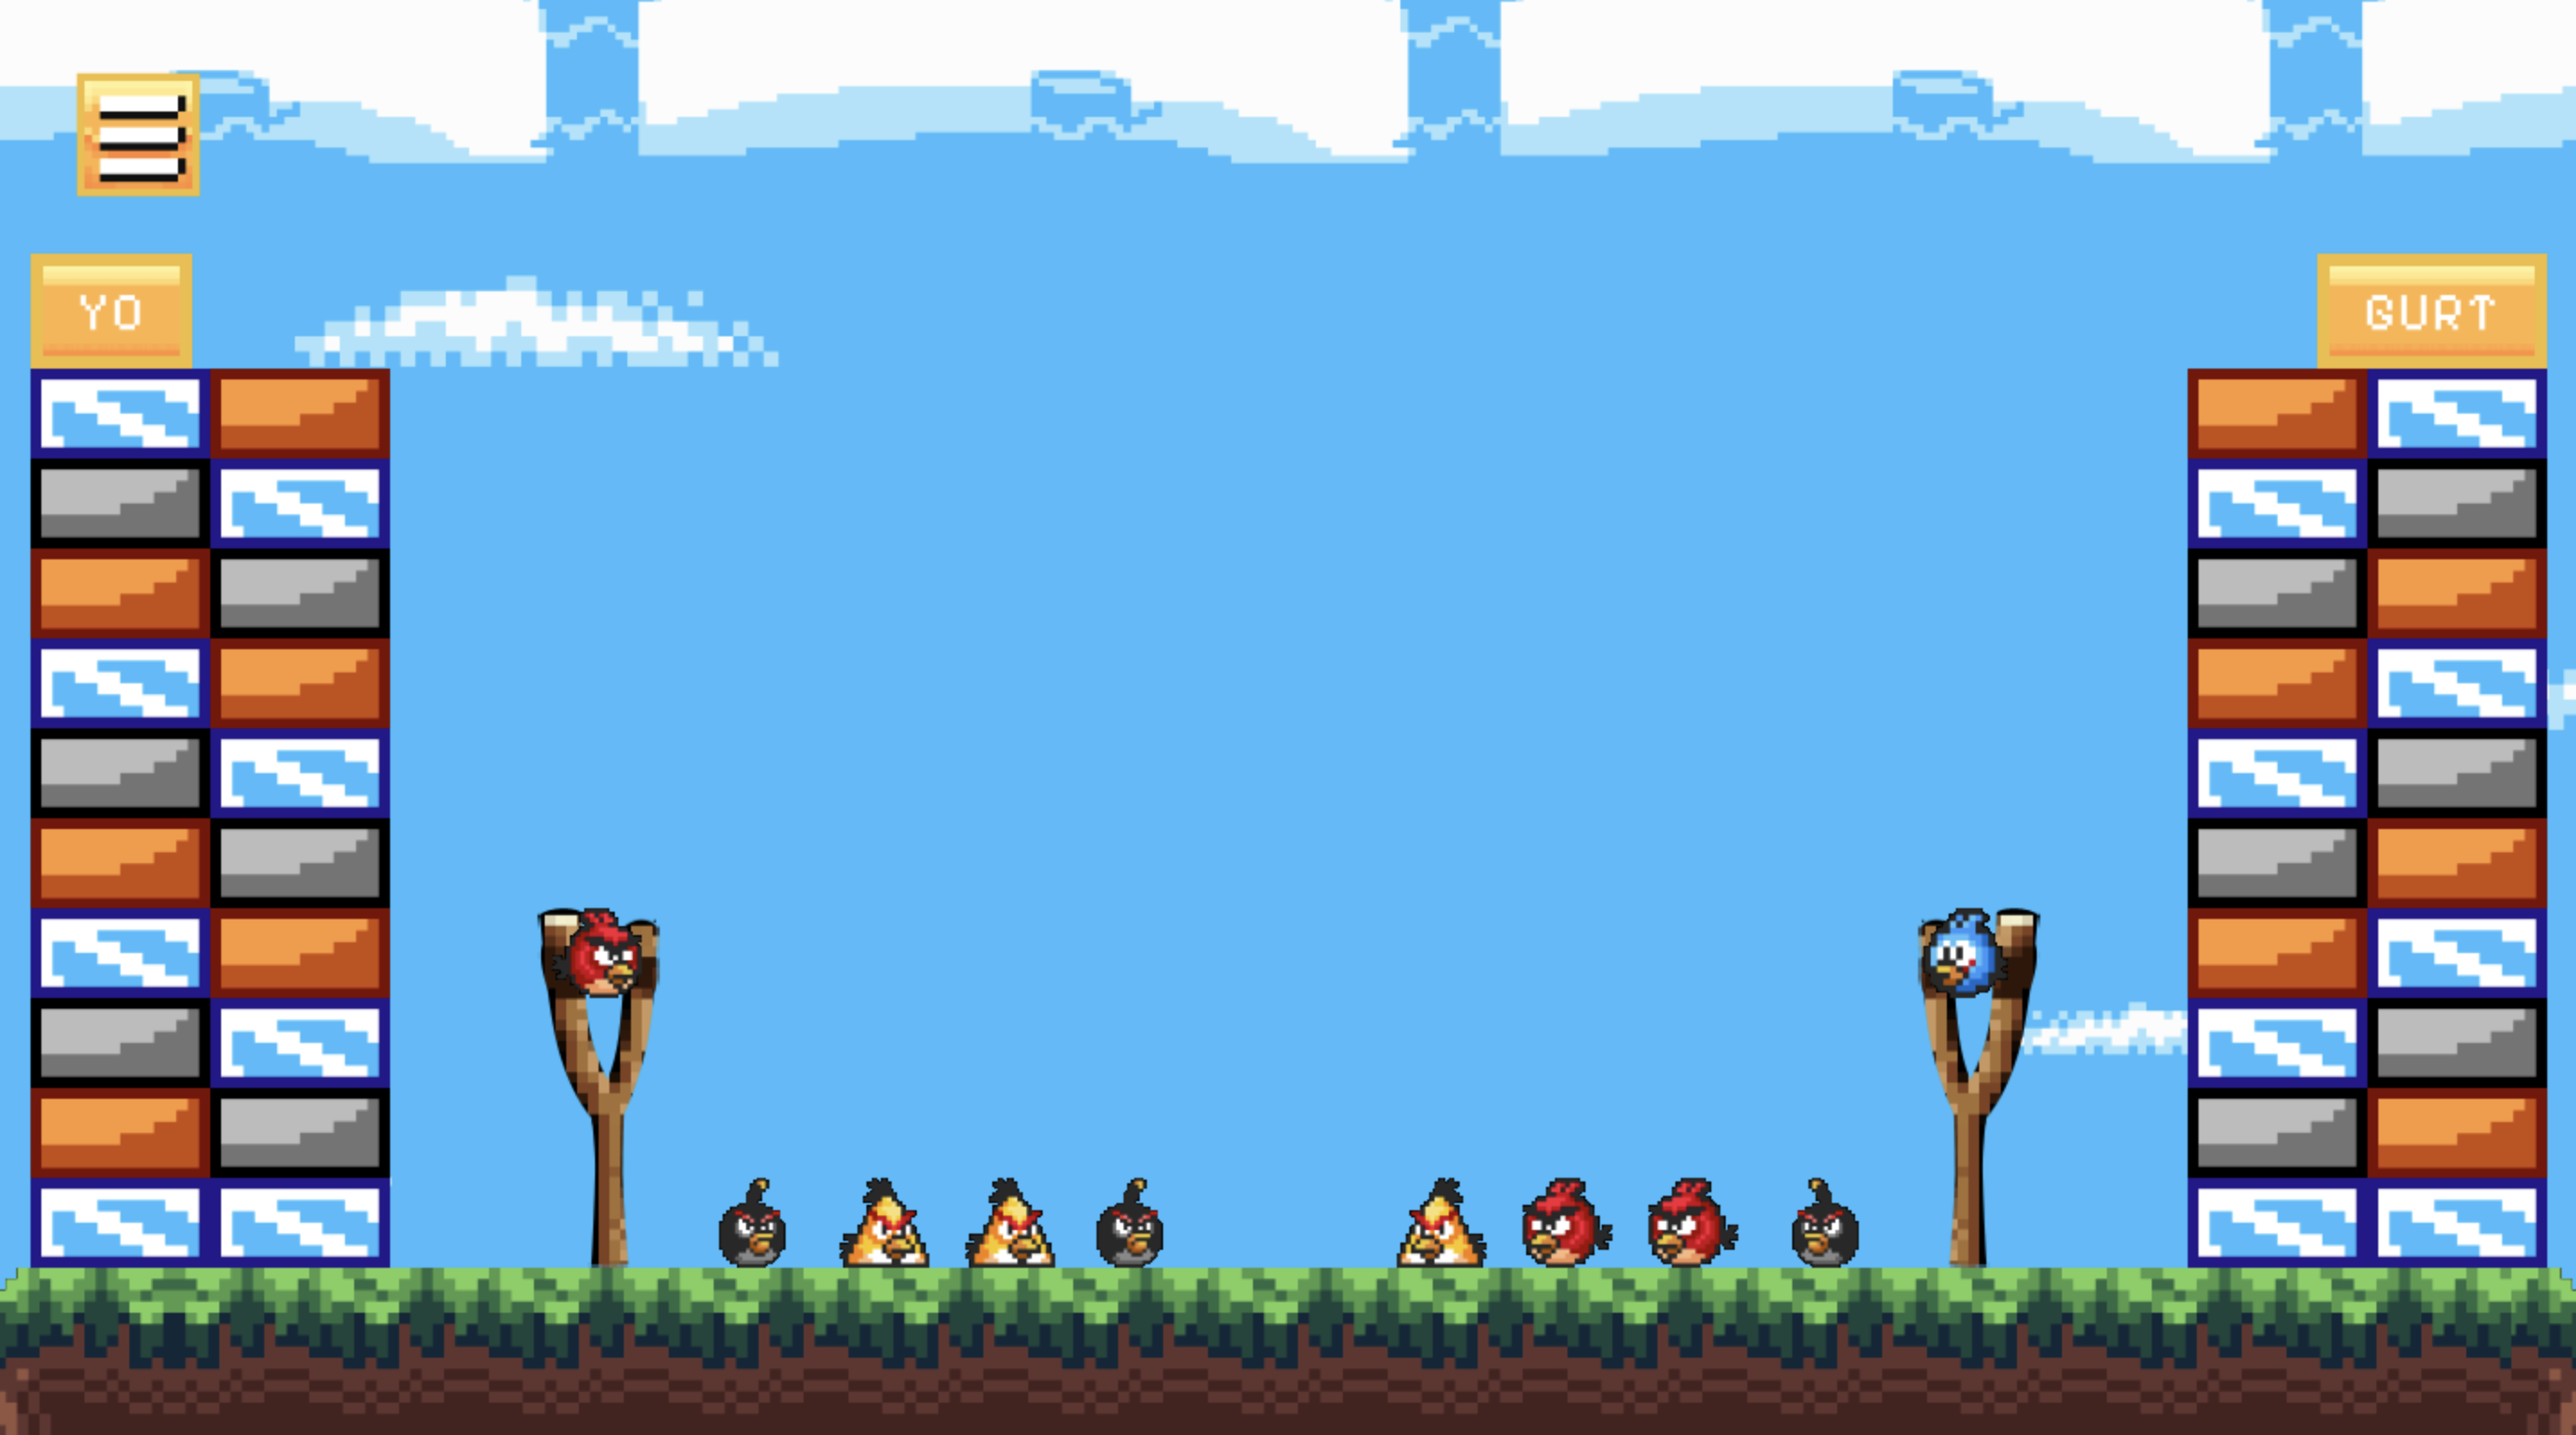
\includegraphics[width=0.5\textwidth]{game.png}
    \caption{Main Gameplay (Two Tower Mode)}
\end{figure}

\subsubsection*{Birds without Special Abilities:}
\begin{itemize}
    \item \textbf{Red Bird} – It does balanced damage (50) to each type of block. \\ Damage - Ice: 50, Wood: 50, Stone: 50
    \item \textbf{Blue Bird} – Damage - Ice: 50, Wood: 25, Stone: 25
    \item \textbf{Yellow Bird} – Damage - Ice: 25, Wood: 50, Stone: 25
    \item \textbf{Black Bird} – Damage - Ice: 25, Wood: 25, Stone: 50
\end{itemize}

\subsubsection*{Birds with Special Abilities:}
These abilities can be triggered mid-flight by pressing a key (e.g., Spacebar).
\begin{itemize}
    \item \textbf{Blue Bird (Splitter)} – Splits into three blue birds mid-air, allowing a spread attack ideal for fragile or widely spaced blocks. \\ Damage - Ice: 50, Wood: 25, Stone: 25
    \item \textbf{Yellow Bird (Speed Boost)} – Accelerates sharply forward when activated, increasing its impact damage significantly. \\ Damage - Ice: 50, Wood: 100, Stone: 50
    \item \textbf{Black Bird (Bomb)} – Explodes mid-air, dealing area-of-effect damage ideal for damaging blocks within a short radius. \\ Damage - Ice: 25, Wood: 25, Stone: 25
\end{itemize}

\subsection{Game Result}
If one player tower is completely demolished, winner's name is displayed on the screen and added to the leaderboard depending on the number of birds used.

\subsection{Leaderboard}
Each mode maintains its own independent leaderboard system, each lists the names of the top 3 winners along with the number of birds used.

\begin{figure}[H]
    \centering
    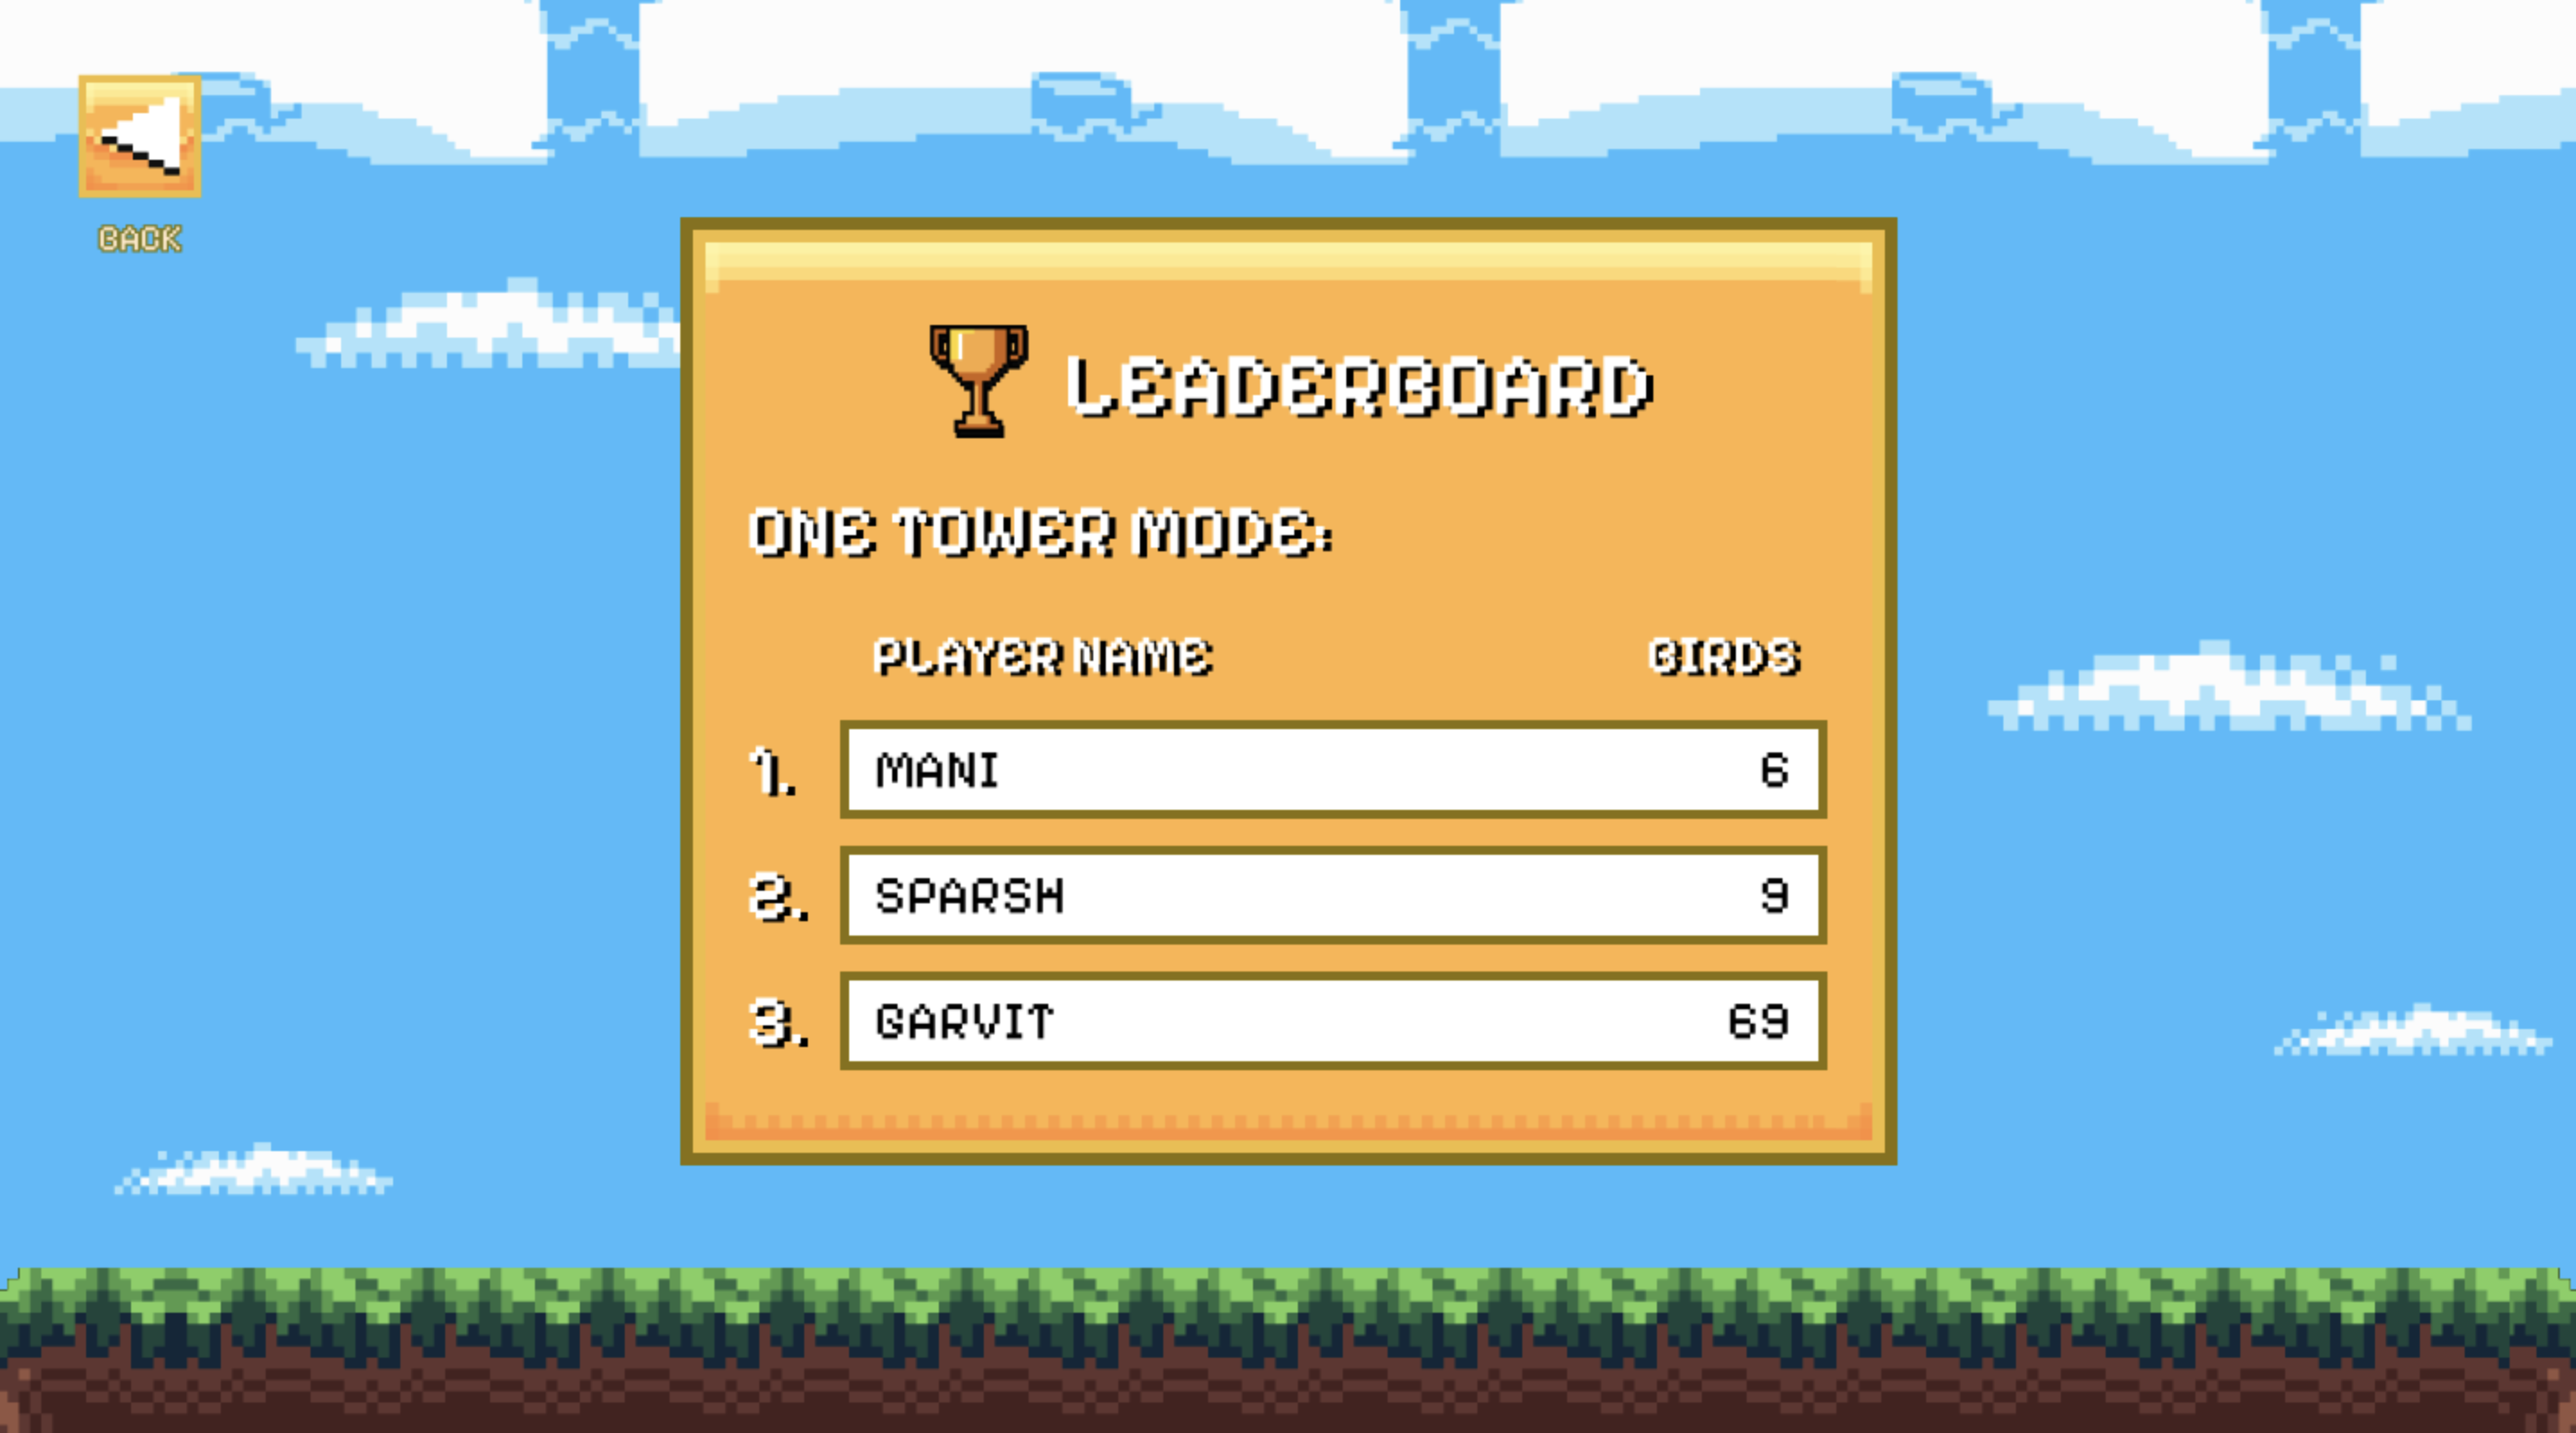
\includegraphics[width=0.5\textwidth]{leaderboard.png}
    \caption{Leaderboard for One Tower Mode}
\end{figure}

\subsection{Settings}
This allows the user to set various game parameters according to their preferences.
\begin{itemize}
    \item \textbf{Background Music} – Allows the user to turn on/off background music.
    \item \textbf{Theme} – A visual toggle that allows users to switch between a \textbf{Day Theme} and a \textbf{Night Theme}.
    \item \textbf{Wind Effect} – Introduces lateral wind forces influencing the trajectory of launched birds.
    \item \textbf{Trajectory Dots} – To aid aiming, the game includes an optional \textbf{Trajectory Guide} system that visually predicts the bird’s initial path after launch.
\end{itemize}

\begin{figure}[H]
    \centering
    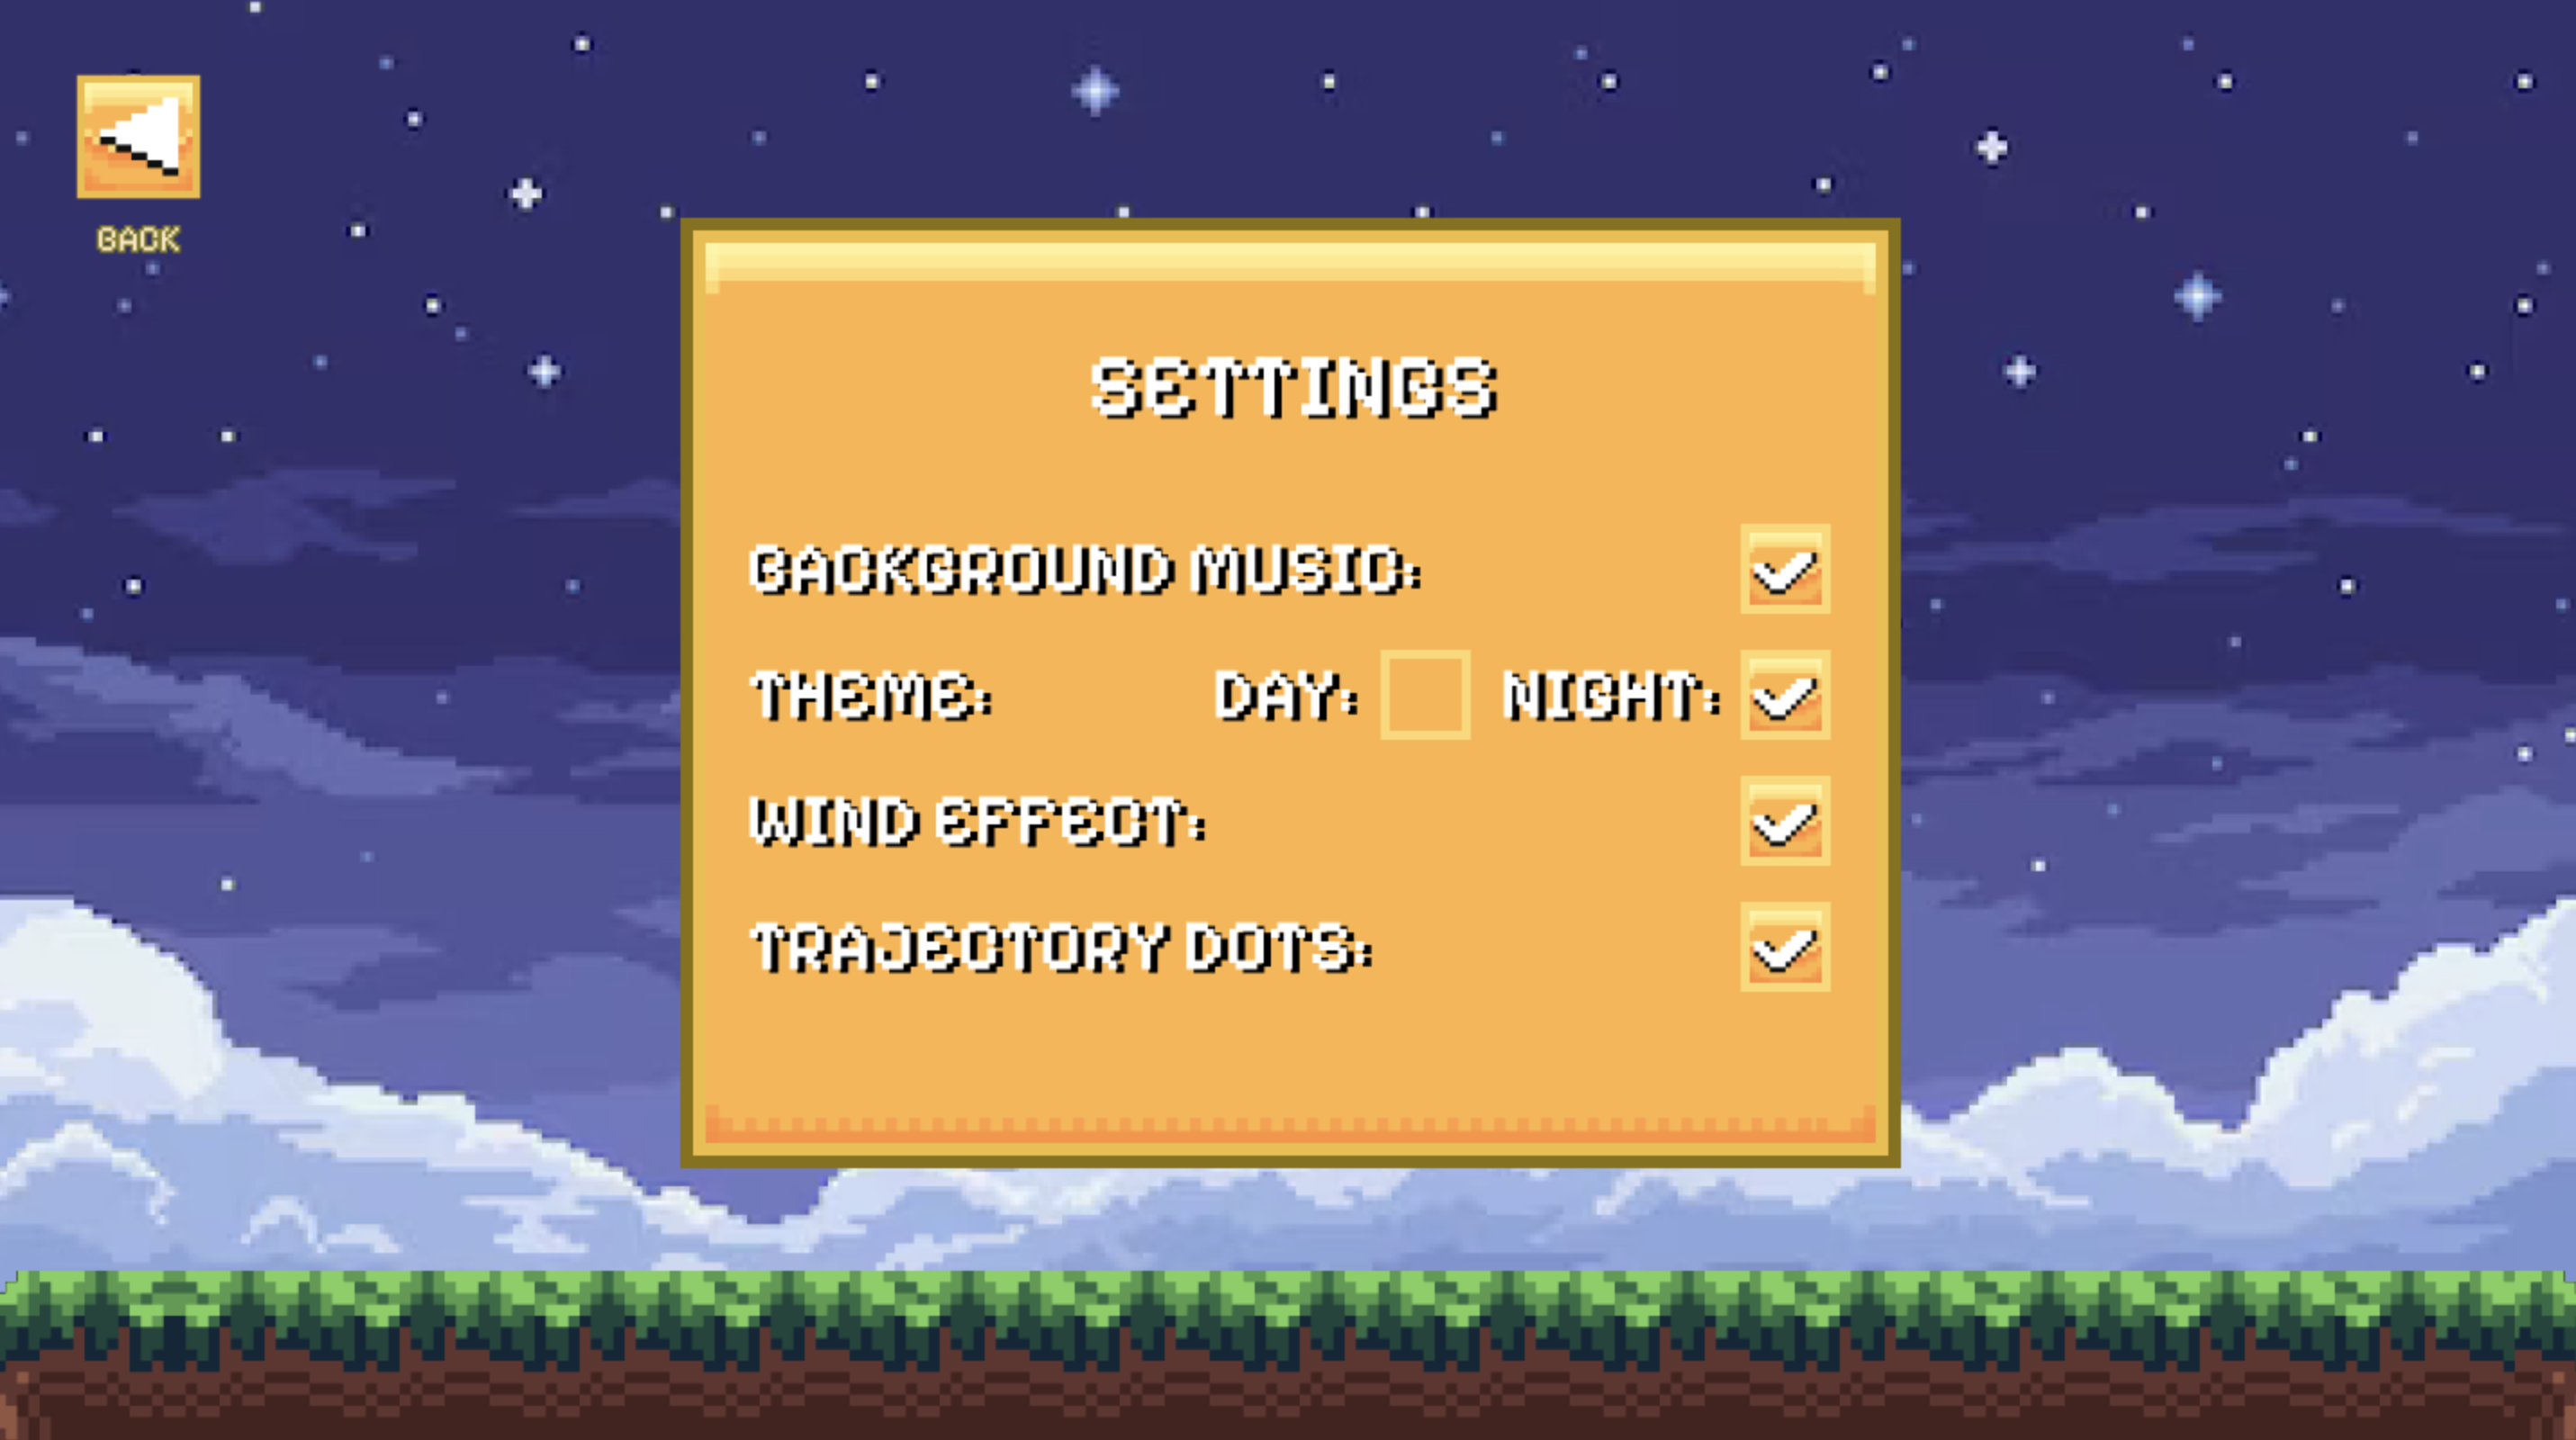
\includegraphics[width=0.5\textwidth]{settings.png}
    \caption{Settings}
\end{figure}

\subsection{Quit}
Players can quit the game by clicking on the quit button.

\section{Customizations}
\begin{itemize}
    \item Themes - Day Theme and Night Theme
    \item Wind - Alters the bird's horizontal velocity
    \item Special abilities - Blue Bird (Splitter), Yellow Bird (Speed Boost), Black Bird (Bomb)
    \item Bird Sounds - Bird launching and special ability sound effects.
    \item Game Modes - One Tower Mode and Two Tower Mode
    \item Guiding Trajectory Dots - To aid aiming (can be enabled/disabled in \textit{Settings})
    \item Dynamic Block Damage Representation - Four distinct sprites that update at 25\% health intervals.
    \item Cloud Animations - Clouds move periodically if wind is enabled.
\end{itemize}

\section{Challenges Faced}
\begin{itemize}
    \item \textbf{Physics Accuracy:} Ensuring realistic projectile motion and collision response without external engines like Pymunk.
    \item \textbf{Bird Launch Smoothness:} Fine-tuning drag mechanics and velocity calculations to eliminate launch jitter.
    \item \textbf{Collision Detection:} Handling bird collisions with blocks and based on which side of block was hit, changing velocity vector of bird.
    \item \textbf{UI Responsiveness:} Creating a responsive interface that transitions cleanly between menus, gameplay, and end states.
\end{itemize}

\section{References}
\begin{itemize}
    \item Pygame Documentation: \url{https://www.pygame.org/docs/}
    \item Pygame CE Documentation: \url{https://pyga.me/docs/}
\end{itemize}

\end{document}
